% !Mode:: "TeX:UTF-8"

\BiChapter{深度学习方法在特征值问题中的应用}{}

这里我们应用深度学习方法来求解椭圆特征值问题。由于特征值问题中,我们要求解的特征函数一般不具有高频震荡的性质,此外,特征值问题的结果随区间变换而改变。这里我们用普通的没有尺度变换的全连接网络求解特征值问题,目的主要是展示深度学习方法在求解特征值问题中的能力。

\BiSection{高维方形区域上的特征值问题}{}

求解椭圆方程特征值问题\ref{prob2},其中参数选取为$a(x)=1$,$c(x)=0$,求解区域为$\Omega = [0, 1]^d$。

问题的最小特征值为$\lambda = d \pi^2$,对应的特征函数
\begin{equation}
u(x) = \prod_{i=1}^{d} \sqrt{2} \sin(\pi x_i)
\end{equation}
我们用Ritz方法求解问题,测试规模为\textbf{1-1000-1000-1000-1000-1}的全连接网络。
激活函数是\textbf{ReLU}。
每次训练区域内部生成\textbf{5000}个点,区域边界生成\textbf{4000}个点。
选取边界惩罚系数为\textbf{1000},归一化惩罚系数为\textbf{10000}。
分别在$d=3$,$d=5$和$d=10$的情况下求解特征值问题。
实验结果如图\ref{f1},图\ref{f2},图\ref{f3}。

在这些图中,图(a)画出了特征值的近似值和真实值随迭代步数变化的图像,图(b)画出了特征函数的近似解和真实解之间的误差。由于高维情况下的特征函数难以画图表示,我们选取两个截面作图。图中,“特征函数1”画出的是在$x_1 = x_2 = \cdots = x_{d-1} = 0.5$截面上的数值解图像,“特征函数2”画出的是在$x_1 = x_2 = \cdots = x_d$对角线上的数值解图像。

\begin{figure}[h]
\centering
\subfigure[特征值]{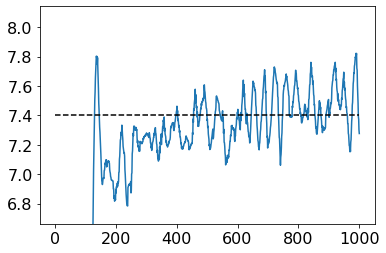
\includegraphics[width=0.3\linewidth]{\fpath report3/lam3d}}
\subfigure[特征函数误差]{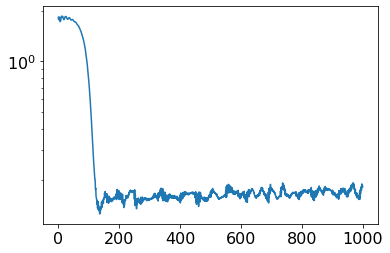
\includegraphics[width=0.3\linewidth]{\fpath report3/err3d}}\\
\subfigure[特征函数1]{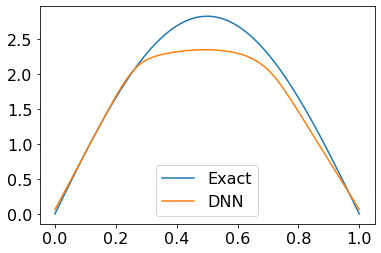
\includegraphics[width=0.3\linewidth]{\fpath report3/samp3d1}}
\subfigure[特征函数2]{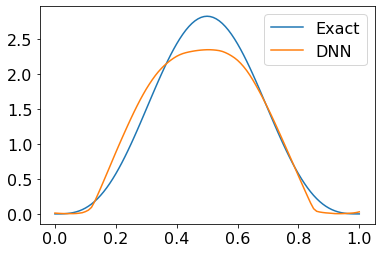
\includegraphics[width=0.3\linewidth]{\fpath report3/samp3d2}}
\caption{高维区域上的实验结果(d=3)}
\label{f1}
\end{figure}

\begin{figure}[h]
\centering
\subfigure[特征值]{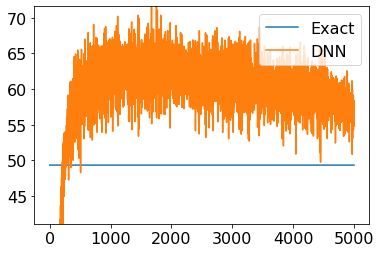
\includegraphics[width=0.3\linewidth]{\fpath report3/lam5d}}
\subfigure[特征函数误差]{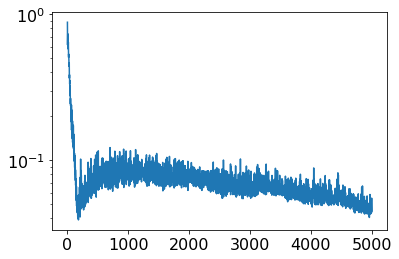
\includegraphics[width=0.3\linewidth]{\fpath report3/err5d}}\\
\subfigure[特征函数1]{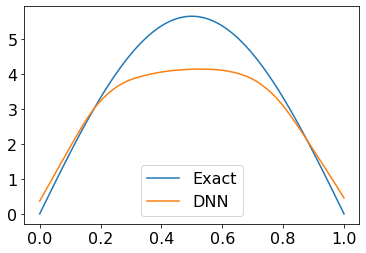
\includegraphics[width=0.3\linewidth]{\fpath report3/samp5d1}}
\subfigure[特征函数2]{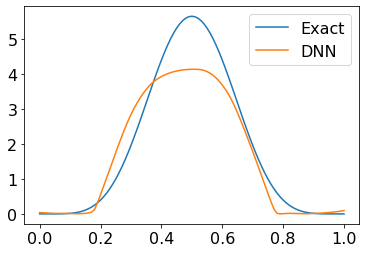
\includegraphics[width=0.3\linewidth]{\fpath report3/samp5d2}}
\caption{高维区域上的实验结果(d=5)}
\label{f2}
\end{figure}

\begin{figure}[h]
\centering
\subfigure[特征值]{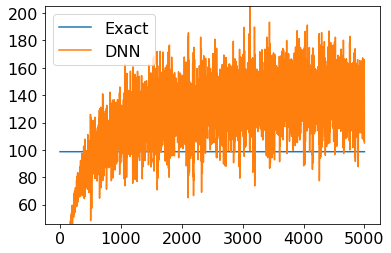
\includegraphics[width=0.3\linewidth]{\fpath report3/lam10d}}
\subfigure[特征函数误差]{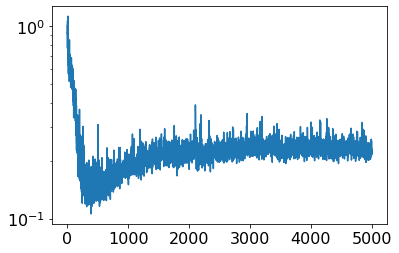
\includegraphics[width=0.3\linewidth]{\fpath report3/err10d}}\\
\subfigure[特征函数1]{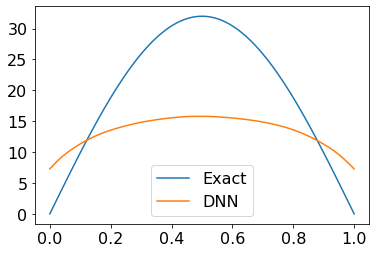
\includegraphics[width=0.3\linewidth]{\fpath report3/samp10d1}}
\subfigure[特征函数2]{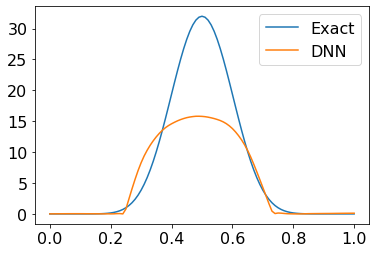
\includegraphics[width=0.3\linewidth]{\fpath report3/samp10d2}}
\caption{高维区域上的实验结果(d=10)}
\label{f3}
\end{figure}

实验中展示了深度学习方法求解高维问题的能力,对于维数很高的问题,传统方法很难应用,但深度学习方法可以给出一些相对可以接受的近似解。但是值得注意的是,随着维度的增高,需要求解得到的目标函数也越来越复杂,这就需要更宽和更深的神经网络来逼近,这同样对计算能力提出了一定的挑战。

\BiSection{变系数的特征值问题}{}

求解椭圆方程特征值问题\ref{prob2},其中参数选取为$a(x)=1$,求解区域为$\Omega = [0, 1]^d$。这里我们把$c(x)$选为分片常数,测试深度学习方法对变系数特征值问题的效果。

\BiSubsection{一维数值实验}{}

首先我们测试一维的情况,测试规模为\textbf{1-200-200-200-1}的全连接网络。
每次训练区域内部生成\textbf{1000}个点,区域边界生成\textbf{200}个点。
边界惩罚系数$\beta_2$为\textbf{1000},归一化惩罚系数$\beta_1$为\textbf{1000}。其它参数相同。

计算结果如图\ref{fb1}。图(a)中画出了势函数的选取,图(b)表示特征值的近似值和真实值随迭代步数变化的图像。图(c)中画出了精确解和深度学习方法给出的近似解的图像。可以看出,在一维的变系数问题上,虽然网络没有刻画出解精确的细节,但是峰值的位置已经可以确定了。

\begin{figure}[h]
\centering
\subfigure[势函数c(x)]{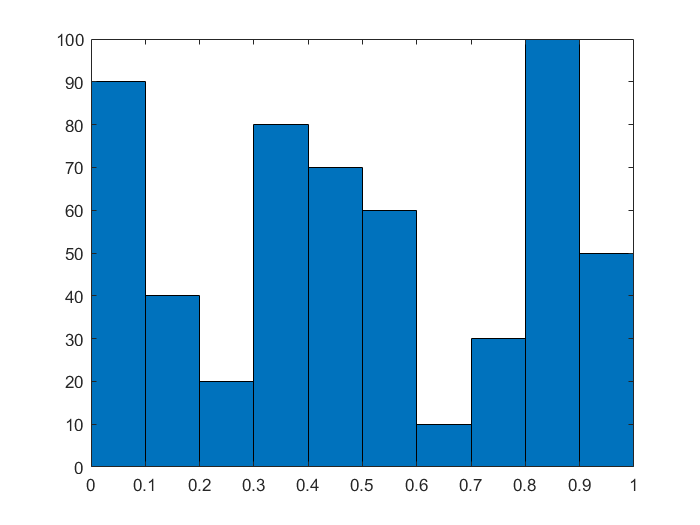
\includegraphics[width=0.3\linewidth]{\fpath report2/V1}}
\subfigure[特征值]{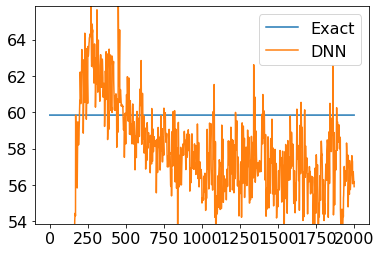
\includegraphics[width=0.3\linewidth]{\fpath report2/lam1}}
\subfigure[特征函数]{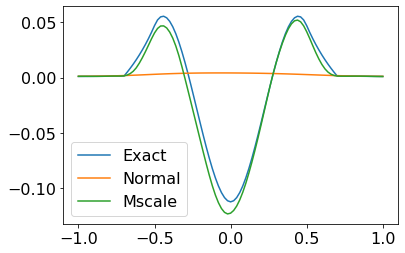
\includegraphics[width=0.3\linewidth]{\fpath report2/samp1}}
\caption{一维变系数方程中的实验结果}
\label{fb1}
\end{figure}

\BiSubsection{二维数值实验}{}

在二维的情况下,我们测试规模为\textbf{1-800-800-800-1}的全连接网络。参数选取为
每次训练区域内部生成\textbf{4000}个点,区域边界生成\textbf{1000}个点。
边界惩罚系数$\beta_2$为\textbf{1000},归一化惩罚系数$\beta_1$为\textbf{10000}。其它参数相同。

计算结果如图\ref{fb3}。图(a)中画出了势函数的选取,图(b)表示特征值的近似值和真实值随迭代步数变化的图像。图(c)和(d)中画出了精确解和深度学习方法给出的近似解的图像。可以看出,二维情况下误差比一维的更大了,但还是在可以接受的范围内。

\begin{figure}[h]
\centering
\subfigure[势函数c(x)]{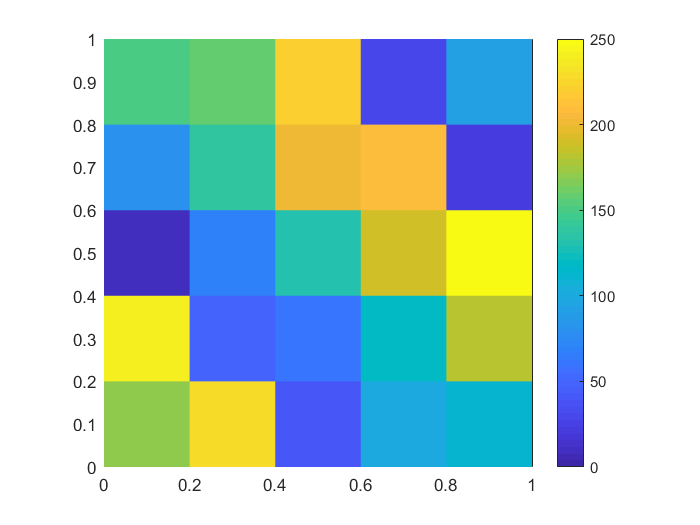
\includegraphics[width=0.3\linewidth]{\fpath report2/V3}}
\subfigure[特征值]{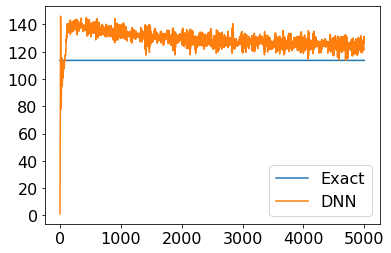
\includegraphics[width=0.3\linewidth]{\fpath report2/lam3}} \\
\subfigure[特征函数参考解]{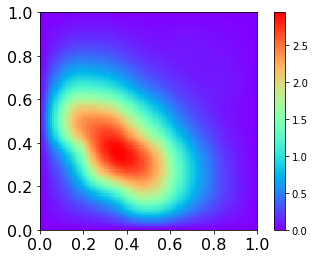
\includegraphics[width=0.3\linewidth]{\fpath report2/samp3r}}
\subfigure[特征函数数值解]{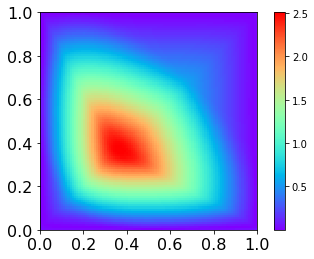
\includegraphics[width=0.3\linewidth]{\fpath report2/samp3n}}
\caption{二维变系数方程中的实验结果}
\label{fb3}
\end{figure}

\BiSection{具有几何奇异性的特征值问题}{}

在椭圆方程特征值问题\ref{prob2}中,参数选取为$a(x)=1$,$c(x)=0$,我们选取不同的求解区域,验证几何奇异性对深度学习方法求解特征值问题的影响。

\BiSubsection{复杂单连通区域}{}

这里的求解区域为一个多边形区域,多边形的顶点依次为$(-1,1) \rightarrow (-1,-1) \rightarrow (1,-1) \rightarrow (1,-0.6) \rightarrow (-0.3,-0.6) \rightarrow (-0.3,0) \rightarrow (0,0) \rightarrow (0,-0.5) \rightarrow (1,-0.5) \rightarrow (1,1) \rightarrow (0.5,1) \rightarrow (0.5,0.3) \rightarrow (-1,1)$。

如图\ref{R1r}为通过matlab的PDE工具箱生成的网格和求解得到的特征函数参考解。问题的最小特征值参考解为$\lambda = 19.2725$。

\begin{figure}[h]
\centering
\subfigure[PDE工具箱生成的网格]{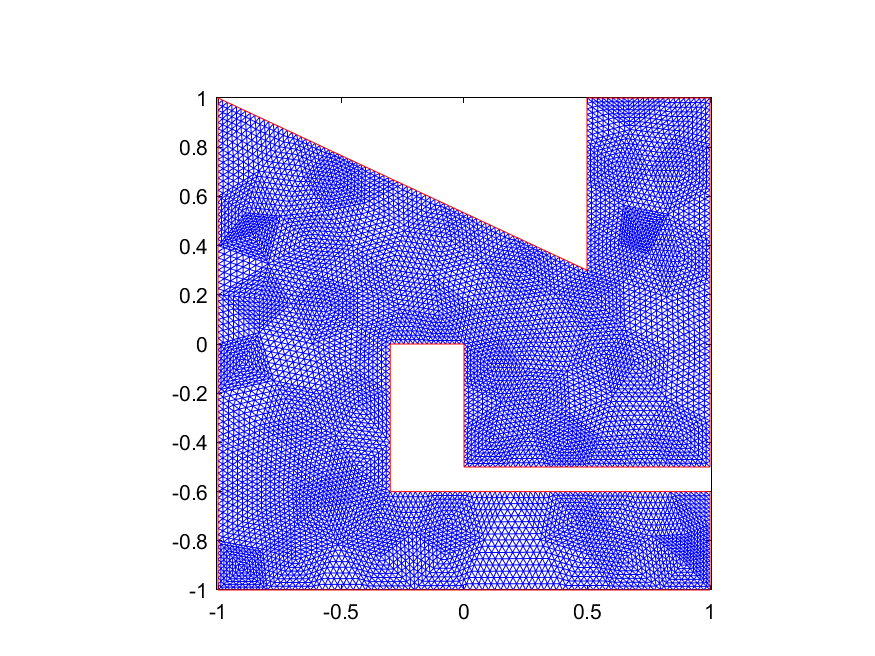
\includegraphics[width=0.35\linewidth]{\fpath report4/R1_m}}
\subfigure[特征函数图像]{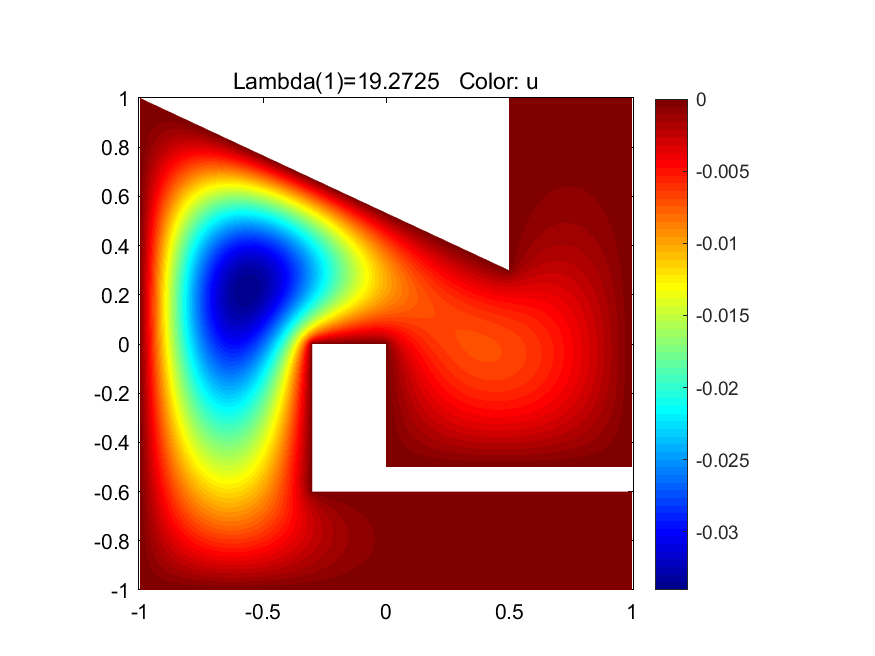
\includegraphics[width=0.35\linewidth]{\fpath report4/R1_l1}}
\caption{参考解图像}
\label{R1r}
\end{figure}

在深度学习方法中,我们测试规模为\textbf{1-800-800-800-1}的全连接网络。
每次训练区域内部生成\textbf{8000}个点,区域边界生成\textbf{2500}个点。
边界惩罚系数$\beta_2$为\textbf{1000},归一化惩罚系数$\beta_1$为\textbf{10000}。
计算结果如图\ref{R1d}。图(a)画出了特征值的近似值和真实值随迭代步数变化的图像,图(b)画出了特征函数的近似解和真实解之间的误差。图(c)画出了迭代5000步后近似解的图像。
可以看出,通过深度学习得到的特征函数近似解和参考解相差不大。在这样的区域上,深度学习方法效果很好。

\begin{figure}[h]
\centering
\subfigure[特征值]{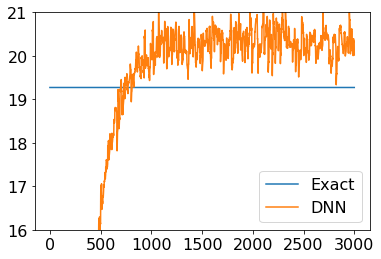
\includegraphics[width=0.3\linewidth]{\fpath report4/R1_lam}}
\subfigure[特征函数误差]{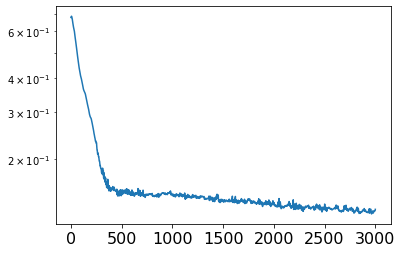
\includegraphics[width=0.3\linewidth]{\fpath report4/R1_err}}
\subfigure[特征函数图像]{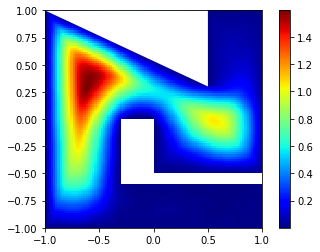
\includegraphics[width=0.3\linewidth]{\fpath report4/R1_DNN}}
\caption{深度学习结果}
\label{R1d}
\end{figure}

\BiSubsection{有孔区域}{}

下面我们求解有孔区域上的特征值问题。求解区域为正方形$[-1,1]^2$挖去三个圆形的洞。洞的圆心和半径依次为
$c_1 = (-0.3, 0.3), r_1 = 0.5, c_2 = (0.6, 0), r_2 = 0.3, c_3 = (-0.1, -0.7), r_3 = 0.2$。

如图\ref{R2r}为通过matlab的PDE工具箱生成的网格和求解得到的特征函数参考姐。问题的最小特征值为$\lambda = 28.8807$。

\begin{figure}[h]
\centering
\subfigure[PDE工具箱生成的网格]{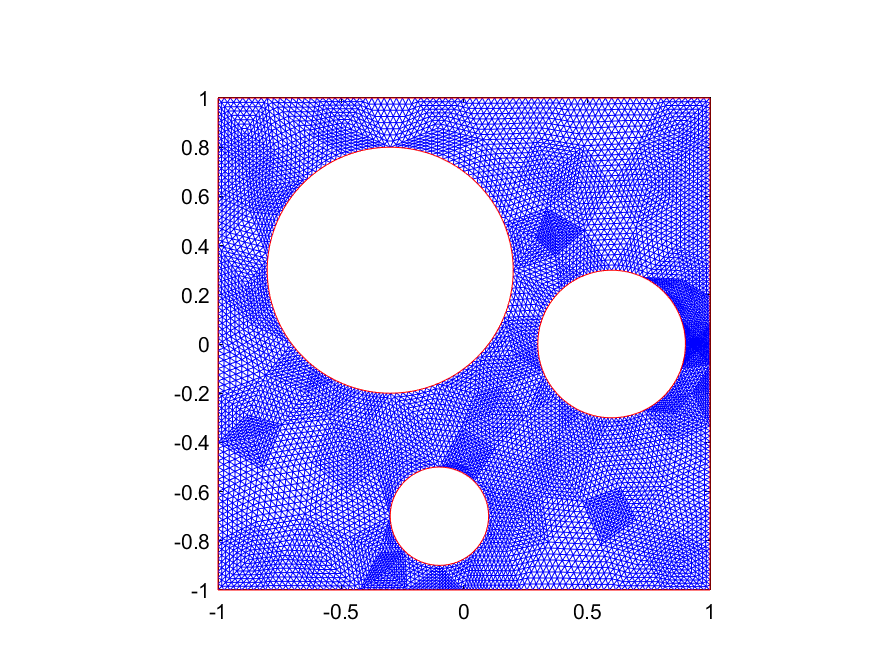
\includegraphics[width=0.35\linewidth]{\fpath report4/R2_m}}
\subfigure[特征函数图像]{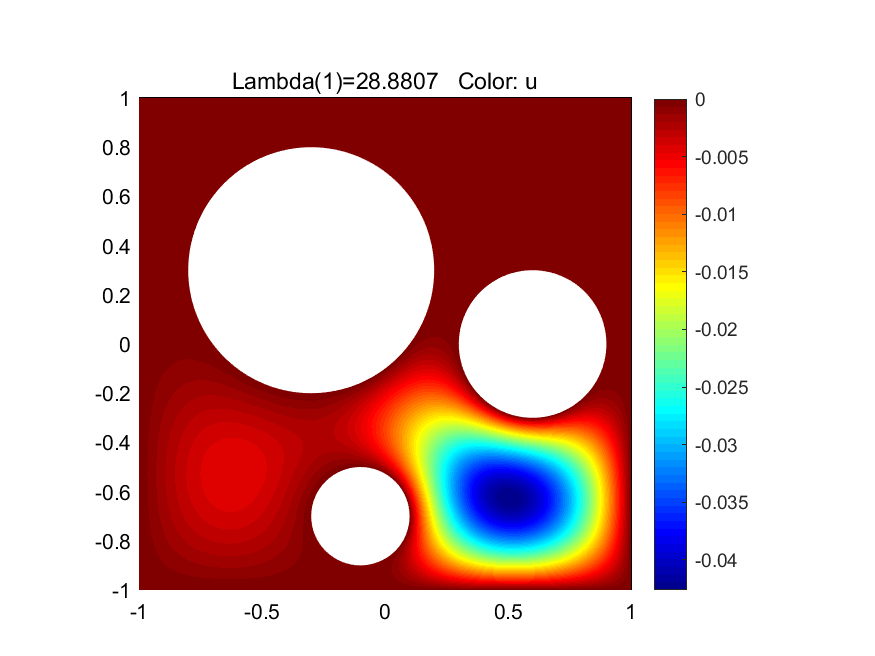
\includegraphics[width=0.35\linewidth]{\fpath report4/R2_l}}
\caption{参考解图像}
\label{R2r}
\end{figure}

在同样的参数下用深度学习方法求解,实验结果如图\ref{R2d}。可以看出,深度学习方法和PDE工具箱中给出的参考解有一定差距,但是特征函数的大致形状和峰的位置都已经被刻画出来了。

\begin{figure}[h]
\centering
\subfigure[特征值]{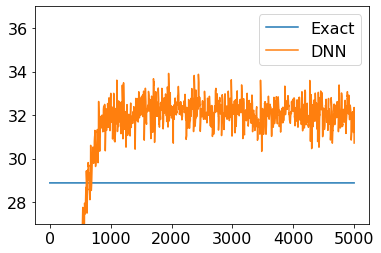
\includegraphics[width=0.3\linewidth]{\fpath report4/R2_lam}}
\subfigure[特征函数误差]{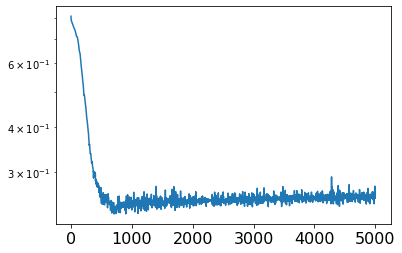
\includegraphics[width=0.3\linewidth]{\fpath report4/R2_err}}
\subfigure[特征函数图像]{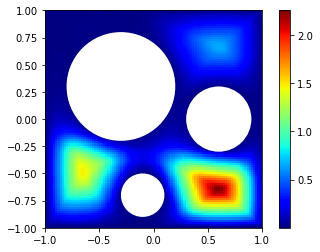
\includegraphics[width=0.3\linewidth]{\fpath report4/R2_DNN}}
\caption{深度学习结果}
\label{R2d}
\end{figure}

\BiSubsection{多孔区域}{}

我们选取求解区域为正方形$[-1,1]^2$挖去$25$个圆形的洞。洞的圆心位于区域内的均匀网格上,半径依次在$0.05,0.15$之间均匀划分。

如图\ref{R3r}为通过matlab的PDE工具箱求解得到的特征函数和网格。最小特征值为$\lambda = 68.9198$。

\begin{figure}[h]
\centering
\subfigure[网格]{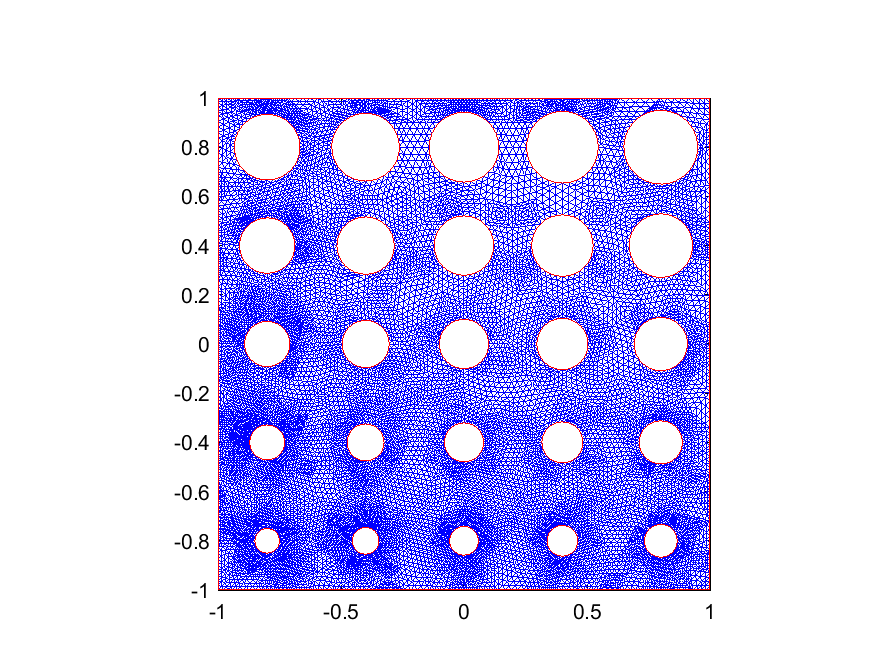
\includegraphics[width=0.35\linewidth]{\fpath report4/R3_m}}
\subfigure[特征函数图像]{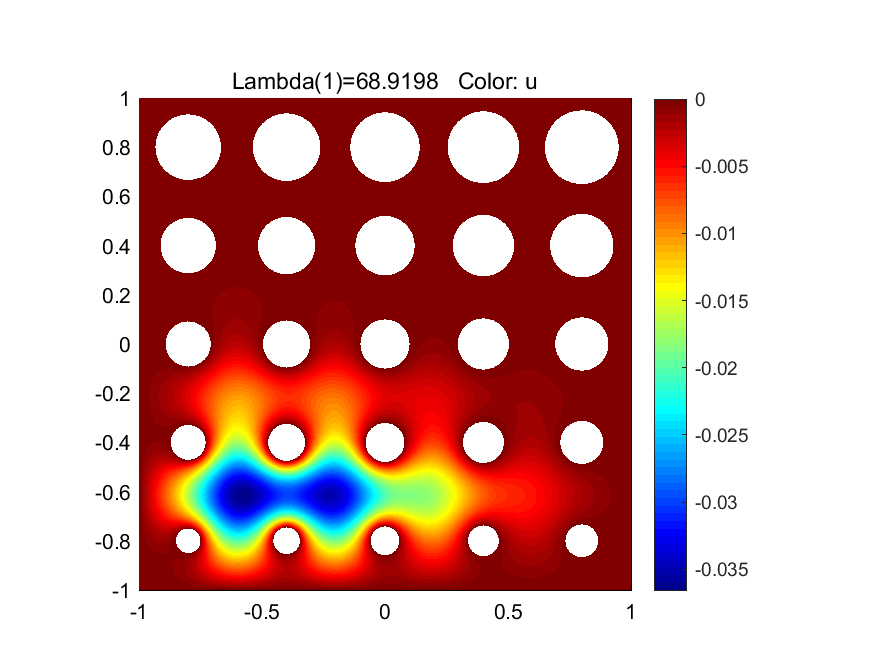
\includegraphics[width=0.35\linewidth]{\fpath report4/R3_l}}
\caption{参考解图像}
\label{R3r}
\end{figure}

在同样的参数下用深度学习方法求解,实验结果如图\ref{R3d}。对于这样复杂的区域,深度学习方法的效果明显变差,几乎完全没有得到正确的结果。这说明深度学习方法在处理一些复杂的特征值问题时,还有很大的改进空间。

\begin{figure}[h]
\centering
\subfigure[特征值]{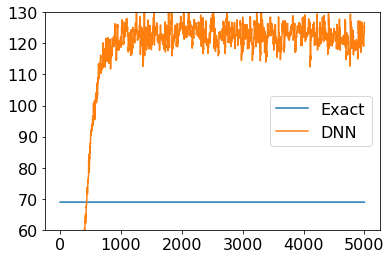
\includegraphics[width=0.3\linewidth]{\fpath report4/R3_lam}}
\subfigure[特征函数误差]{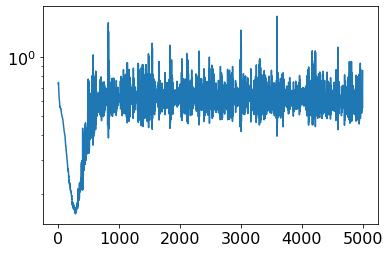
\includegraphics[width=0.3\linewidth]{\fpath report4/R3_err}}
\subfigure[特征函数图像]{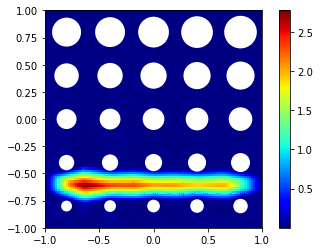
\includegraphics[width=0.3\linewidth]{\fpath report4/R3_DNN}}
\caption{深度学习结果}
\label{R3d}
\end{figure}
